\documentclass{article}

\usepackage{graphicx}
\usepackage{tikz}
\usepackage{tikzsymbols}
\usetikzlibrary{calc,patterns,shapes.geometric}
\pagestyle{empty}
\usepackage[margin=0pt]{geometry}
\geometry{papersize={14in,12in}}

\def\centerarc[#1](#2)(#3:#4:#5){\draw[#1] ($(#2)+({#5*cos(#3)},{#5*sin(#3)})$) arc (#3:#4:#5);}

\begin{document}
	\begin{figure}
		\centering
		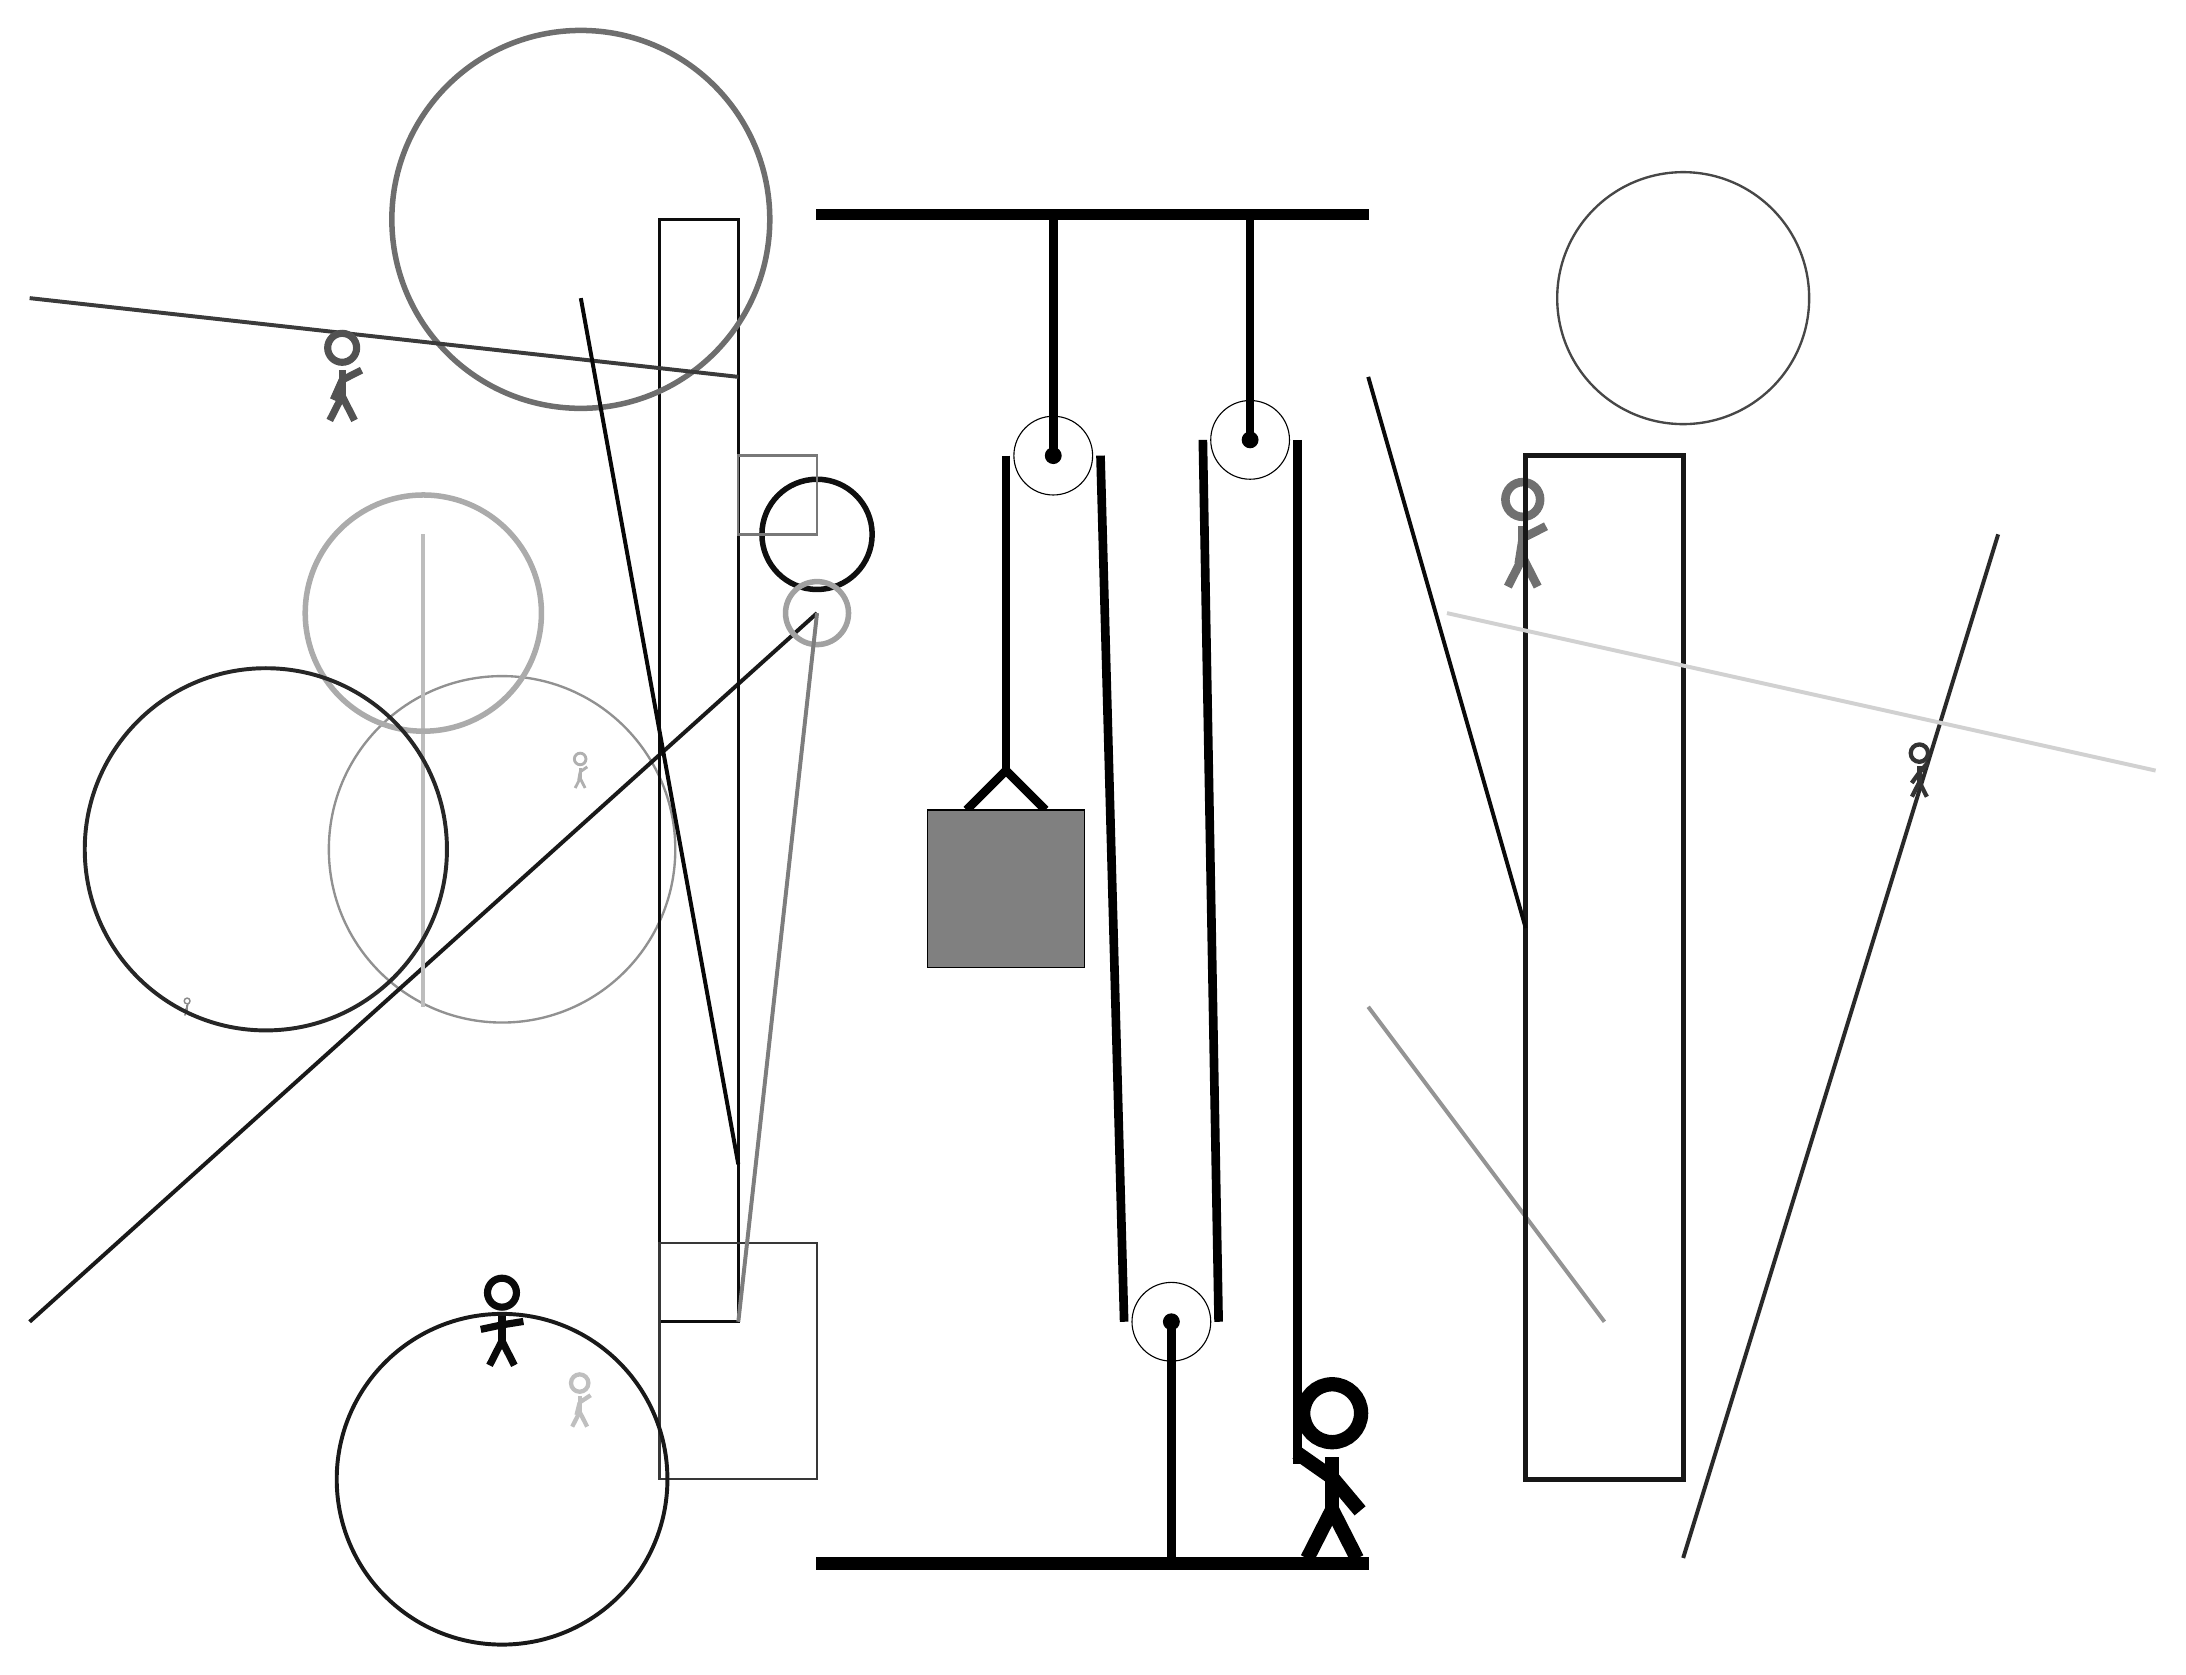
\begin{tikzpicture}
			%%%%% START %%%%%
			
			\draw[fill=black] (-2, 14) rectangle (5, 14.125);
			
			\draw (1, 11) circle (0.5);
			\draw[fill=black] (1, 11) circle (0.1);
			\draw[line width=1.1mm]  (1, 14) -- (1, 11);
			
			\draw[fill=white](2.5, 0) circle (0.5);
			\draw[fill=black] (2.5, 0) circle (0.1);
			\draw[line width=1.1mm]  (2.5, -3) -- (2.5, 0);
			
			\draw[fill=white](3.5, 11.2) circle (0.5);
			\draw[fill=black] (3.5, 11.2) circle (0.1);
			\draw[line width=1.1mm] (3.5, 14) -- (3.5, 11.2);
			
			\draw[line width=1.1mm] (-0.1, 6.5) -- (0.4, 7.0) -- (0.9, 6.5);
			\draw[fill=black!50] (-0.6, 6.5) rectangle (1.4, 4.5);
			
			\node[line width=0.7mm, color=black!56] at (7, 10) {\Strichmaxerl[6][81][27]};
			
			\draw[line width=0.5mm, color=black!42](8, 0) -- (5, 4);
			\draw [line width=0.3mm, color=black!43](-6, 6) circle (2.2);
			\draw [line width=0.3mm, color=black!72](9, 13) circle (1.6);
			
			\draw[line width=0.5mm, color=black!90](-2, 9) -- (-12, 0);
			
			\draw [line width=0.7mm, color=black!94](-2, 10) circle (0.7);
			\draw[line width=0.5mm, color=black!26](-7, 4) -- (-7, 10);
			\node[line width=0.6mm, color=black!96] at (-6, 0) {\Strichmaxerl[5][12][9]};
			\draw[line width=0.6mm, color=black!91] (7, -2) rectangle (9, 11);
			
			\draw[line width=0.4mm, color=black!95] (-4, 14) rectangle (-3, 0);
			\draw[line width=0.5mm, color=black!96](7, 5) -- (5, 12);
			\draw[line width=0.5mm, color=black!84](9, -3) -- (13, 10);
			\draw [line width=0.7mm, color=black!33](-7, 9) circle (1.5);
			\draw[line width=0.3mm, color=black!78] (-4, -2) rectangle (-2, 1);
			\draw[line width=0.3mm, color=black!53] (-2, 10) rectangle (-3, 11);
			\draw [line width=0.7mm, color=black!57](-5, 14) circle (2.4);
			\node[line width=0.7mm, color=black!25] at (-5, -1) {\Strichmaxerl[3][76][33]};
			\draw[line width=0.5mm, color=black!77](-3, 12) -- (-12, 13);
			\draw [line width=0.7mm, color=black!37](-2, 9) circle (0.4);
			\draw[line width=0.5mm, color=black!18](6, 9) -- (15, 7);
			\node[line width=0.5mm, color=black!46] at (-10, 4) {\Strichmaxerl[1][50][76]};
			
			\node[line width=0.7mm, color=black!68] at (-8, 12) {\Strichmaxerl[5][66][27]};
			\node[line width=0.5mm, color=black!31] at (-5, 7) {\Strichmaxerl[2][80][35]};
			\node[line width=0.3mm, color=black!80] at (12, 7) {\Strichmaxerl[3][54][49]};
			\draw[line width=0.5mm, color=black!51](-3, 0) -- (-2, 9);
			\draw[line width=0.5mm, color=black!97](-5, 13) -- (-3, 2);
			\draw [line width=0.5mm, color=black!90](-6, -2) circle (2.1);
			\draw[line width=0.6mm, color=black!68] (-3, 11) rectangle (-3, 11);
			\draw [line width=0.5mm, color=black!85](-9, 6) circle (2.3);
			
			\draw [line width=0.7mm, color=black!43](-5, 13) circle (0.0);
			
			\draw[line width=1.1mm] (0.4, 11) -- (0.4, 7.0);
			\centerarc[line width=1.1mm](1, 11)(0:180:0.6);
			\draw[line width=1.1mm](1.6, 11) -- (1.9, 0);
			\centerarc[line width=1.1mm](2.5, 0)(180:360:0.6);
			\draw[line width=1.1mm](3.1, 0) -- (2.9, 11.2);
			\centerarc[line width=1.1mm](3.5, 11.2)(0:180:0.6);
			\draw[line width=1.1mm](4.1, 11.2) -- (4.1, -1.8);
			
			\node at (4.5, -1.9) {\Strichmaxerl[10][-35][-50]};
			
			\draw[fill=black] (-2, -3) rectangle (5, -3.15);
			
			%%%%% END %%%%%
		\end{tikzpicture}
	\end{figure}	
\end{document}